\begin{problem}
Find the best least squares approximation from the space of polynomials of degree at most one to $f(x) = x^2, \, x \in [0,1]$. Plot the result together with the original function. Plot the error function. Calculate $\lVert f - p^*\rVert$ and $\lVert p^*\rVert$.
\end{problem}

\begin{solution}
We know from the characterization theorem that given a linear subspace $(\mathcal{A} \equiv \mathcal{P}_1)$ of a Hilbert space $(\mathcal{B} \equiv \mathcal{C}[0,1])$ then $p^* \in \mathcal{A}$ is the best least squares approximation to $f \in \mathcal{B}$ if and only if the error $e^* = f - p^*$ satisfies:
\begin{equation*}
\langle e^*,p \rangle = 0, \quad \forall p \in \mathcal{A}
\end{equation*}
As we can write the polynomial as $p^* = \sum_{i=0}^n c_i^* \Phi_i$ where $\Phi_i$ are the basis functions we have that to be the best approximation we need to satisfy $\langle \Phi_i, f-p^* \rangle=0$ that is:
\begin{equation*}
\sum_{j=0}^n \langle \Phi_i,\Phi_j\rangle c_j^* = \langle \Phi_i,f\rangle
\end{equation*}
this expression is called normal equations. Then we have the theorem that says if $\mathcal{A}$ is a linear subspace of  a Hilbert space $\mathcal{B}$ spanned by $\{\Phi_0 \ldots \Phi_n\}$ where $\langle \Phi_i,\Phi_j \rangle = 0$ if $i \neq j$ then the least squares best approximation from $\mathcal{A}$ to $f \in \mathcal{B}$ is:
\begin{equation}
p^*(x) = \sum_{j=0}^n \frac{\langle \Phi_j, f\rangle}{\lVert\Phi_j\rVert_2^2}\Phi_j
\label{bestlsq}
\end{equation}
And to make the basis orthogonal, we use the Gramm-Schmidt method. Let us now apply this two theorems to our function $f(x) = x^2, \, x\in[0,1]$. Take the basis functions $\{1,x\}$ and make them orthogonal:
\begin{align*}
\Phi_0 &= 1 \\
\Phi_1 &=x\Phi_0 - \alpha_0\Phi_0
\end{align*}
Where $\alpha_0 = \frac{\langle \Phi_0, x\Phi_0 \rangle}{\lVert \Phi_0 \rVert_2^2}$. This gives us that $\Phi_1 = (x-1/2)$. Now let us compute the coefficients:
\begin{align*}
c_0^* &= \frac{\langle 1,x^2 \rangle}{\lVert 1 \rVert_2^2}=\frac{1}{3}\\
c_1^* &= \frac{\langle x-1/2, x^2 \rangle}{\lVert x-1/2\rVert_2^2} = 1
\end{align*}
When we plug in this data into equation \ref{bestlsq} we get that our best approximation polynomial is $p^*(x) = x-1/6$. we can see this in Figure \ref{bestlsqfigure}.
\begin{figure}[h]
\centering 
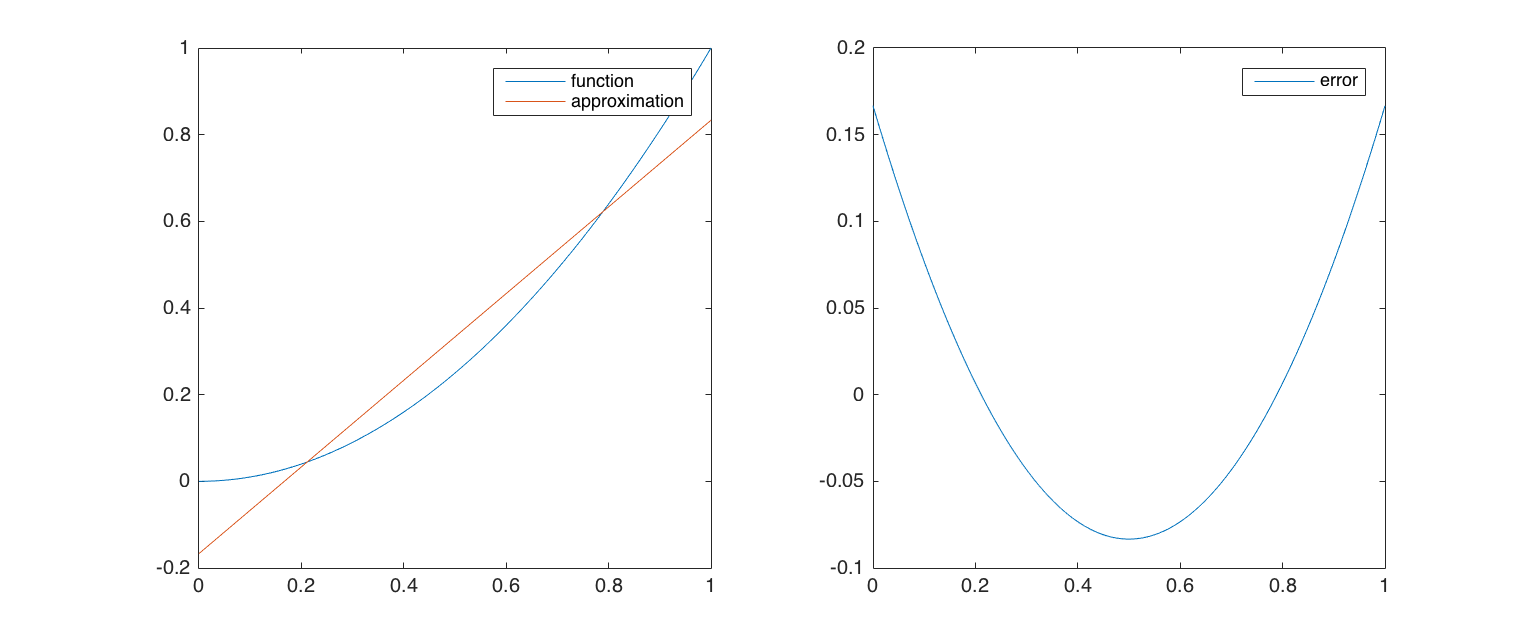
\includegraphics[scale = 0.25]{bestlsqx2.png}
\caption{ plot of the function $x^2$ approximated by $x-1/6$ and error}
\label{bestlsqfigure}
\end{figure}
Finally we are asked to compute the norm of the error:
\begin{equation*}
\lVert x^2-x+1/6\rVert_2 = \sqrt{\int_0^1 (x^2-x+1/6)^2\, dx}=\frac{\sqrt{5}}{30}
\end{equation}
and the norm of $p^*$
\begin{equation*}
\lVert x-1/6 \rVert_2 = \sqrt{\int_0^1 (x-1/6)^2 \, dx} = \frac{7}{36}
\end{equation}
\end{solution}

%%% Local Variables:
%%% mode: latex
%%% TeX-master: "report"
%%% End:
